\documentclass[12pt]{article}

\usepackage{lmodern}
\usepackage[utf8]{inputenc}
\usepackage[T1]{fontenc}
\usepackage[french]{babel}
\usepackage{url}
\usepackage{graphicx}
\graphicspath{ {./img/} }

\title{\textbf{Analyse de données d’eye-tracking en Réalité Virtuelle}}
\author{\Large{Adonis Stavridis}}
\date{Février 2021}

\begin{document}

% ----------------------------------------------------------------------------
% TITLEPAGE
% ----------------------------------------------------------------------------

\maketitle
\tableofcontents
\pagebreak

% ----------------------------------------------------------------------------
% INTRODUCTION
% ----------------------------------------------------------------------------

\section{Introduction}
L'eye-tracking \cite{wiki:eye_tracking}, ou oculométrie, est une technologie
assez récente qui détermine la position du regard d'un individu. Des capteurs
spéciaux envoient des rayons infrarouges vers les yeux d'un individu et ceux-ci
sont réfléchis, leur permettant ainsi de déterminer ses mouvements oculaires
sur un écran. Elle établie alors une nouvelle interface entre Homme et machine
et est devenue aujourd'hui une technologie principale dans des études liées au
système visuel humain, à la psychologie, au marketing et design. Elle est en
fait dèjà très utilisée dans les jeux vidéos. Un domaine où cette technologie
reste encore peu developpée est la réalité virtuelle.

\bigskip
Déterminer la position du regard d'un individu sur un écran permet d'effectuer
des études quantitatives et qualitatives sur de multiples supports, et ainsi
comprendre les comportements humains dans différentes situations. L'eye-tracking
s'avère donc être très pratique pour étudier sur un document par exemple, les
zones qui sont le plus attrayantes et celles qui le sont moins. Cependant,
certaines études ont besoin d'un environment plus réalistes. La réalité
virtuelle ajoute une nouvelle couche d'immersion, permettant à un individu de
se sentir et agir de façon plus réaliste. Ainsi, la réalité virtuelle
permettrait de livrer des résultats beaucoup plus fiables pour certains
domaines, et ainsi aider à l'avancement des recherches sur le comportement
humain.

% ----------------------------------------------------------------------------
% MATERIEL
% ----------------------------------------------------------------------------

\section{Capteurs d'oculométrie}

Pour l'instant, les meilleurs produits liés à l'eye-tracking sont ceux crées
par l'entreprise Tobii \cite{tobii} et HTC Vive \cite{htc_vive_pro_eye}. Elles
proposent des solutions dans plusieurs domaines, des capteurs simples pouvant
être utilisés pour suivre les mouvements sur un écran, des solutions plus
professionnelles pour effectuer des captures dans le monde réel, mais aussi des
produits pour des individus qui nécessitent de l'assistance.

\bigskip
Le capteur le plus basique est une barre à placer en dessous ou au dessus d'un
écran, qui va donc capturer les mouvements oculaires d'un individu et déterminer
la position de son regard sur cet écran. Ce capteur permet d'enregistrer toutes
les données afin de les étudier et effectuer des analyses statistiques. C'est un
produit très pratique, mais laisse peu de liberté de mouvement. Des nouveaux
capteurs d'oculométrie ont éte intégrés à des casques de réalité virtuelle,
pour profiter du mouvement libre dans un monde tri-dimensionnel.

\begin{figure}[htpb]
  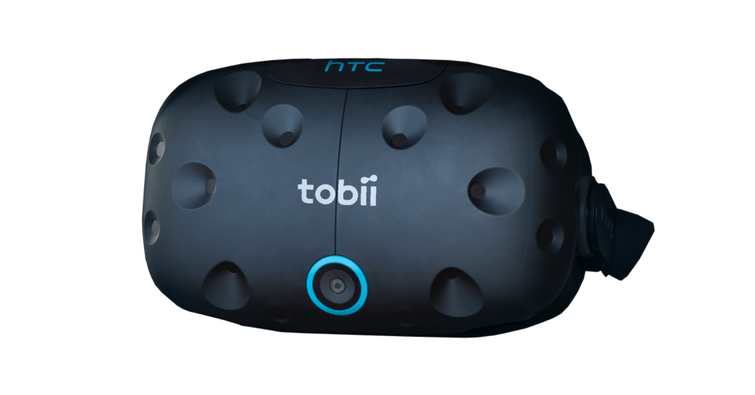
\includegraphics[width=\textwidth,keepaspectratio=true]{tobiivr.png}
  \caption{Casque de réalité virtuelle Tobii VR}
\end{figure}

L'ajout de l'eye-tracking dans la réalité virtuelle permet essentielment de
faire du rendu fovéal \cite{wiki:foveated_rendering} : les yeux ne se
focalisent qu'en une seule région tandis que le reste du champ visuel est flou.
Cette méthode de rendu propose d'effectuer un rendu de très haute qualité à la
région de focalisation mais une qualité de rendu moins important dans les reste
du champ périphérique. La réalité virtuelle a souvent besoin de beaucoup de
puissance de calcul, et donc cette technique de rendu associée avec
l'eye-tracking permettrait de faire des gains en puissance de calcul mais aussi
en qualité de rendu, en plus des fonctionnalités de tout capteur basique.

\bigskip
Tout le matériel de niveau professionnel est déjà présent. Cependant ces produits sont assez récents et donc assez chers.

% ----------------------------------------------------------------------------
% LOGICIELS
% ----------------------------------------------------------------------------

\section{Logiciels}

Plusieurs logiciels existent déjà afin d'effectuer de l'oculométrie avec une
webcam/camera basique. Certains sont open-source et gratuits. Effectuer une
comparaison de ces logiciels, permettrait de comprendre les avantages et
inconvénients de chacune.

\subsection{PyGaze}

\subsection{GazeParser}

% ----------------------------------------------------------------------------
% CONCLUSION
% ----------------------------------------------------------------------------

\section{Conclusion}

% ----------------------------------------------------------------------------
% BIBLIOGRAPHIE
% ----------------------------------------------------------------------------

\pagebreak
\bibliographystyle{unsrt}
\bibliography{recherches}

\end{document}
